\documentclass{beamer}

% For more themes, color themes and font themes, see:
% http://deic.uab.es/~iblanes/beamer_gallery/index_by_theme.html
%
\mode<presentation>
{
  \usetheme{default}       % or try default, Darmstadt, Warsaw, ...
  \usecolortheme{default} % or try albatross, beaver, crane, ...
  \usefonttheme{serif}    % or try default, structurebold, ...
  \setbeamertemplate{navigation symbols}{}
  \setbeamertemplate{caption}[numbered]
} 

\usepackage[german]{babel}
\usepackage[utf8x]{inputenc}
\usepackage{chemfig}
\usepackage[version=3]{mhchem}
\usepackage{listings}
\usepackage{graphicx}

% On Overleaf, these lines give you sharper preview images.
% You might want to `comment them out before you export, though.
\usepackage{pgfpages}
\pgfpagesuselayout{resize to}[%
  physical paper width=8in, physical paper height=6in]

% Here's where the presentation starts, with the info for the title slide
\title{Schema.org Injector}
\author{Stefan Haberl, Mathias Meinschad}
\institute{STI Innsbruck}
\date{14. Dezember 2016}

\begin{document}

\begin{frame}
  \titlepage
\end{frame}

\begin{frame}{Übersicht}
  \tableofcontents
\end{frame}

\section{Projekt}

\begin{frame}{Projekt}
Entwicklung einer Typo3 Extension, welches schema.org annotations in die Webseite injiziert.
Dabei sollen JSON-LD Dateien eingelesen werden und in die passende Webseite injiziert werden ("Code injection").


\begin{block}{Anforderungen:}
\begin{itemize}
\item Alle Seiten sollen von einer JSON-LD Datei verändert werden.
\item Verschiedene Kategorien sollen von verschiedene JSON-LD Dateien verändert werden.
\item Eine Seite soll von einer bestimmten JSON-LD Datei verändert werden.
\end{itemize}
\end{block}
\end{frame}


\section{Typo3}

\begin{frame}{Typo3}
\begin{block}{Was ist Typo3?}
\begin{itemize}
\item Typo3 ist ein Open Source Content Managment System
\item Entwickler: Kasper Skårhøj
\item Erscheinungsjahr: 1998
\item Aktuelle Version: 8.4.1 (22. November 2016)
\item Verwendete Sprachen: PHP, SQL und JavaScript
\end{itemize}
\end{block}
\begin{block}{Was ist ein Content Managment System (CMS)?}
Ein CMS ist eine Software zur gemeinschaftlichen Erstellung, Bearbeitung und Organisation von Inhalten.
\end{block}

\end{frame}


\section{JSON-LD}

\begin{frame}[fragile]
\frametitle{JSON-LD}
\begin{block}{Was ist ein JSON-LD file?}
JSON-LD (Linked Data) ist eine Empfehlung des W3C, weltweit verknüpfte Daten im JSON Format einzubetten. Dabei wird das klassische Name-Wert-Paar durch sogenannte Keywords ergänzt.
\end{block}

\begin{block}{Beispielcode JSON-LD}
\begin{lstlisting}
<script type="application/ld+json">
{
  "@context": "http://schema.org/",
  "@type": "Person",
  "name": "Albert Einstein"
}
</script>
\end{lstlisting}
\end{block}
\end{frame}

\section{Probleme}

\begin{frame}{Bisherige Probleme}
\begin{itemize}
\item Keine Erfahrung mit Typo3
\item Schwache Dokumentation für Extension Entwicklung
\item Sehr kleine Community
\item Schlechtes Basiswissen über PHP
\item Funktionsweise von Typo3: Code Injection, HTML Generierung
\end{itemize}
\end{frame}


\section{Fortschritt}

\begin{frame}{Fortschritt}
\begin{figure}[ht]
\centering
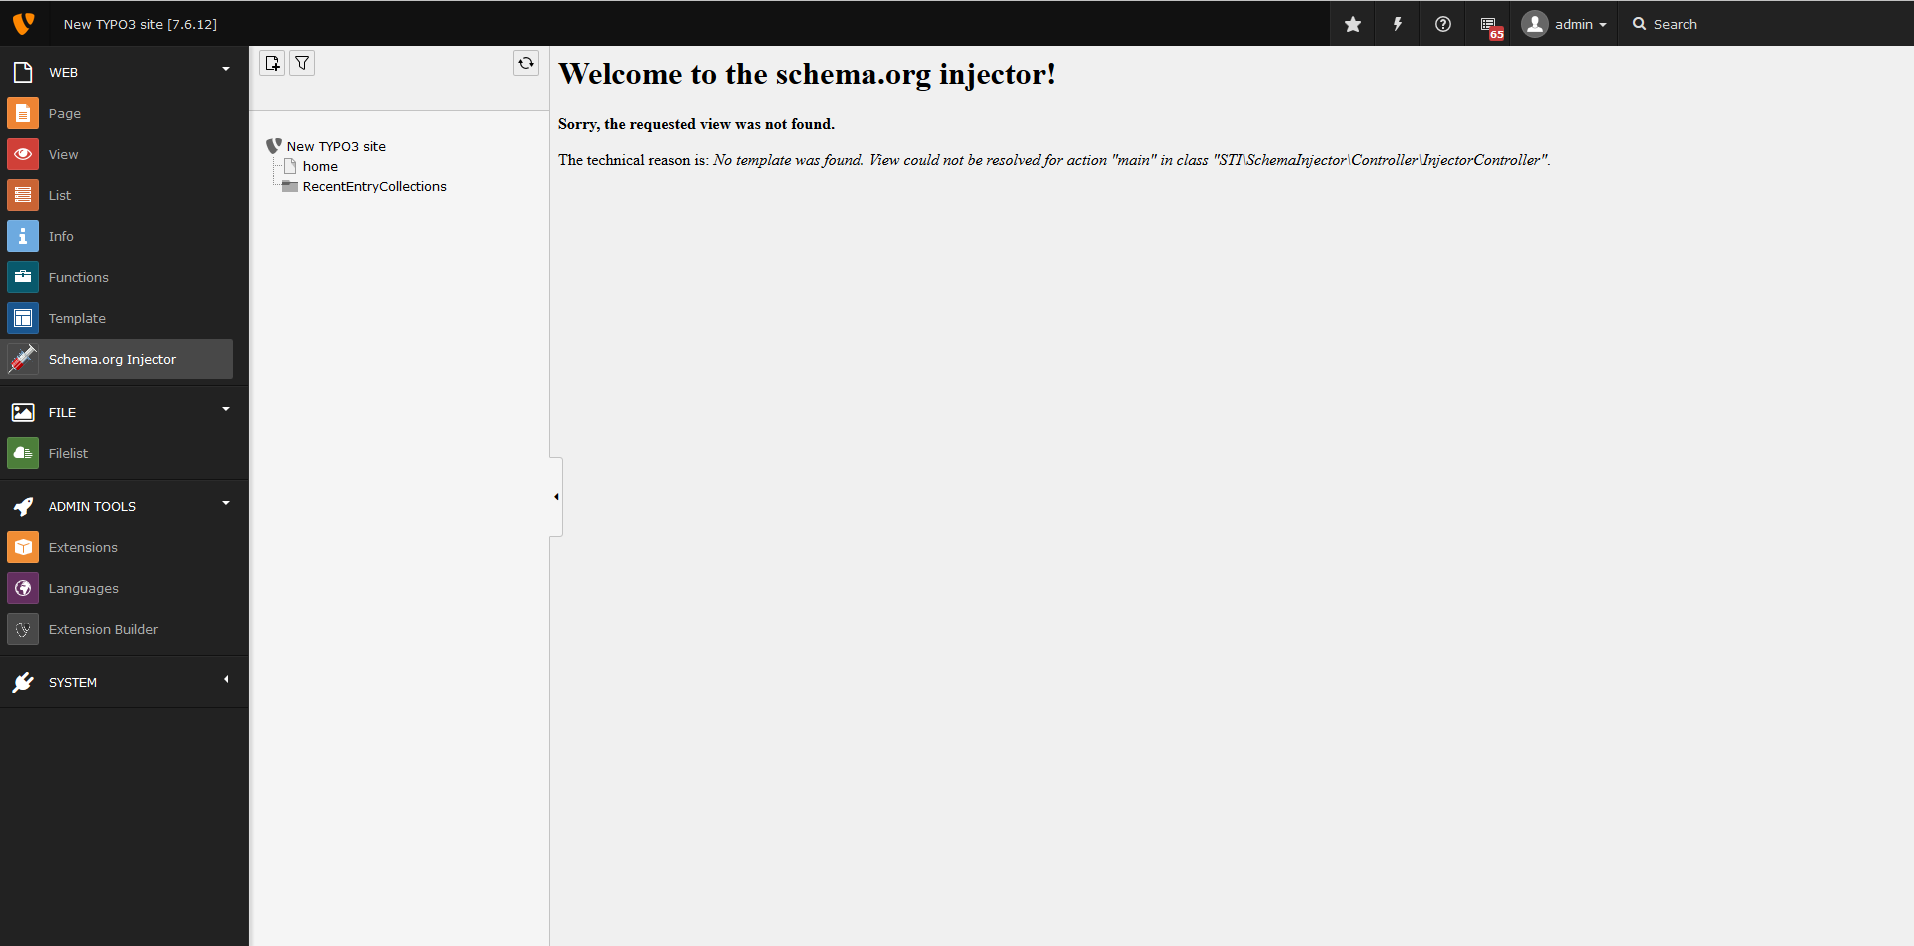
\includegraphics[width=1.0\textwidth]{example_image.png}
\caption{Abbildung der Oberfläche unserer Extension}
\end{figure}
\end{frame}

\end{document}